\documentclass[11pt]{article}
\usepackage{amsmath, amssymb, amsthm}
\usepackage{geometry}
\usepackage{hyperref}
\usepackage{tikz}
\usetikzlibrary{arrows.meta, positioning}
\geometry{margin=1in}

\title{Notes 00 \\ Review of Statistics: \\ Regression Analysis}
\author{DATA 000: Advanced Computational Methods in Education and the Social Sciences}
\date{Alexander \\ Spring 2026}

\begin{document}

\maketitle

\tableofcontents

\section{Introduction}

\textbf{Regression analysis} is a powerful statistical method for modeling and analyzing the relationship between a dependent variable (outcome) and one or more independent variables (predictors). In education and the social sciences, regression is used to explain, predict, and infer relationships among variables such as test scores, income, attitudes, and behaviors\ [2][5][7][8].

\section{Key Concepts and Terminology}

\begin{itemize}
    \item \textbf{Dependent variable ($Y$):} The outcome we want to explain or predict.
    \item \textbf{Independent variable(s) ($X$):} The predictor(s) or factors thought to influence $Y$.
    \item \textbf{Regression coefficient ($b$ or $\beta$):} Quantifies the relationship between $X$ and $Y$.
    \item \textbf{Intercept ($a$ or $\beta_0$):} The expected value of $Y$ when all $X$ variables are zero.
    \item \textbf{Residual:} The difference between observed and predicted values ($e_i = y_i - \hat{y}_i$).
\end{itemize}

\section{Simple Linear Regression}

\subsection{Model and Formula}

Models the relationship between a single independent variable $X$ and a dependent variable $Y$:

\[
Y = a + bX + \varepsilon
\]
where:
\begin{itemize}
    \item $Y$ = dependent variable
    \item $X$ = independent variable
    \item $a$ = intercept
    \item $b$ = slope (change in $Y$ for a one-unit change in $X$)
    \item $\varepsilon$ = error term
\end{itemize}

\subsection*{Visualization: Scatterplot with Regression Line}
\begin{center}
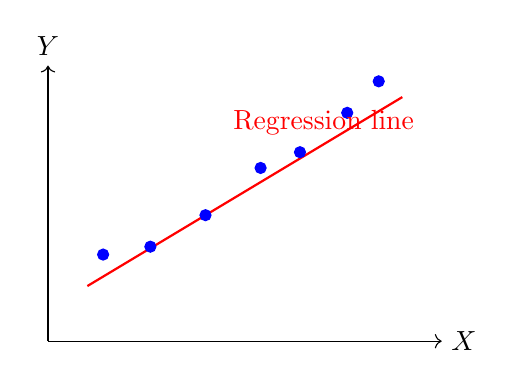
\begin{tikzpicture}[scale=1]
  % Axes
  \draw[->] (0,0) -- (5,0) node[right] {$X$};
  \draw[->] (0,0) -- (0,3.5) node[above] {$Y$};
  % Regression line
  \draw[thick, red] (0.5,0.7) -- (4.5,3.1);
  % Data points
  \foreach \x/\y in {0.7/1.1, 1.3/1.2, 2/1.6, 2.7/2.2, 3.2/2.4, 3.8/2.9, 4.2/3.3} {
    \filldraw[blue] (\x,\y) circle (2pt);
  }
  % Label
  \node[red, above] at (3.5,2.5) {Regression line};
\end{tikzpicture}
\end{center}

\subsection{Interpretation}

- The slope $b$ shows the expected change in $Y$ for each unit increase in $X$.
- The intercept $a$ is the predicted $Y$ when $X=0$ (may not always be meaningful).

\subsection{Example: Education (with Solution)}

\textbf{Scenario:} A researcher examines the relationship between hours studied ($X$) and test score ($Y$) for 5 students:

\begin{tabular}{c|ccccc}
Hours ($X$) & 2 & 4 & 6 & 8 & 10 \\
Score ($Y$) & 65 & 70 & 78 & 85 & 90 \\
\end{tabular}

\textbf{Step 1:} Calculate means: $\bar{X} = 6$, $\bar{Y} = 77.6$

\textbf{Step 2:} Compute slope:

\[
b = \frac{\sum (X_i - \bar{X})(Y_i - \bar{Y})}{\sum (X_i - \bar{X})^2} = \frac{(2-6)(65-77.6) + \ldots + (10-6)(90-77.6)}{(2-6)^2 + \ldots + (10-6)^2}
\]
\[
\sum (X_i - \bar{X})(Y_i - \bar{Y}) = (-4)(-12.6) + (-2)(-7.6) + (0)(0.4) + (2)(7.4) + (4)(12.4) = 50.4 + 15.2 + 0 + 14.8 + 49.6 = 130
\]
\[
\sum (X_i - \bar{X})^2 = 16 + 4 + 0 + 4 + 16 = 40
\]
\[
b = 130 / 40 = 3.25
\]

\textbf{Step 3:} Compute intercept:

\[
a = \bar{Y} - b\bar{X} = 77.6 - 3.25 \times 6 = 77.6 - 19.5 = 58.1
\]

\textbf{Regression equation:} $\hat{Y} = 58.1 + 3.25X$

\textbf{Interpretation:} Each additional hour studied predicts a 3.25 point increase in test score.

\section{Multiple Linear Regression}

\subsection{Model and Formula}

Models the relationship between $Y$ and two or more independent variables:

\[
Y = a + b_1 X_1 + b_2 X_2 + \cdots + b_n X_n + \varepsilon
\]

\begin{itemize}
    \item $X_1, X_2, \ldots, X_n$ are independent variables.
    \item $b_1, b_2, \ldots, b_n$ are the coefficients for each predictor.
\end{itemize}

\subsection{Interpretation}

- Each coefficient $b_j$ represents the expected change in $Y$ for a one-unit increase in $X_j$, holding other variables constant.

\subsection{Example: Social Science (with Solution)}

\textbf{Scenario:} Predicting college GPA ($Y$) from high school GPA ($X_1$) and SAT score ($X_2$):

\[
\text{Regression output:} \quad \hat{Y} = 0.5 + 0.6 X_1 + 0.002 X_2
\]

\textbf{Interpretation:}
- For each one-point increase in high school GPA, college GPA increases by 0.6 (holding SAT constant).
- For each 100-point increase in SAT, college GPA increases by $0.002 \times 100 = 0.2$ (holding high school GPA constant).

\section{Logistic Regression}

\subsection{Purpose and Model}

Used when the dependent variable is binary (e.g., pass/fail, yes/no):

\[
\log\left( \frac{p}{1-p} \right) = a + b_1 X_1 + b_2 X_2 + \cdots + b_n X_n
\]

where $p$ is the probability of the outcome of interest.

\subsection*{Visualization: Logistic Curve}
\begin{center}
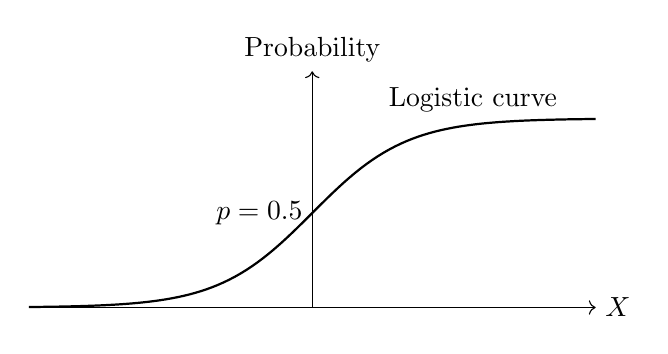
\begin{tikzpicture}[scale=1.2]
  \draw[->] (-3,0) -- (3,0) node[right] {$X$};
  \draw[->] (0,0) -- (0,2.5) node[above] {Probability};
  \draw[thick, domain=-3:3, samples=100] plot (\x, {2/(1+exp(-2*\x))});
  \node at (1.7,2.2) {Logistic curve};
  \draw[dashed] (0,0) -- (0,1);
  \node[left] at (0,1) {$p=0.5$};
\end{tikzpicture}
\end{center}

\subsection{Interpretation}

- Coefficients show the effect of predictors on the \emph{log odds} of the outcome.
- Exponentiating coefficients gives odds ratios.

\subsection{Example: Education (with Solution)}

\textbf{Scenario:} Predicting whether a student passes (1) or fails (0) a test based on hours studied ($X$):

\[
\log\left( \frac{p}{1-p} \right) = -2 + 0.5 X
\]

\textbf{Interpretation:} For each additional hour studied, the odds of passing increase by $e^{0.5} \approx 1.65$ times.

\textbf{Probability for $X=4$:}
\[
\log\left( \frac{p}{1-p} \right) = -2 + 0.5 \times 4 = 0
\]
\[
\frac{p}{1-p} = 1 \implies p = 0.5
\]

\section{Diagnostics and Model Checking}

\subsection{Assumptions (Linear Regression)}

\begin{itemize}
    \item Linearity: Relationship between $X$ and $Y$ is linear.
    \item Independence: Observations are independent.
    \item Homoscedasticity: Constant variance of residuals.
    \item Normality: Residuals are normally distributed.
    \item No multicollinearity: Predictors are not highly correlated.
\end{itemize}

\subsection*{Visualization: Residual Plot}
\begin{center}
\begin{tikzpicture}[scale=1]
  % Axes
  \draw[->] (0,0) -- (5,0) node[right] {Fitted values};
  \draw[->] (0,-2) -- (0,2.5) node[above] {Residuals};
  % Points (random scatter)
  \foreach \x/\y in {0.7/0.5, 1.3/0.8, 2/0.2, 2.7/-0.7, 3.2/-1.1, 3.8/0.3, 4.2/1.1} {
    \filldraw[blue] (\x,\y) circle (2pt);
  }
  % Zero line
  \draw[dashed] (0,0) -- (4.5,0);
  \node at (4,2) {No pattern: good fit};
\end{tikzpicture}
\end{center}

\subsection{Common Diagnostics}

\begin{itemize}
    \item \textbf{Residual plots:} Check for patterns (should be random).
    \item \textbf{Normal Q-Q plot:} Check residual normality.
    \item \textbf{Variance Inflation Factor (VIF):} Check multicollinearity.
    \item \textbf{$R^2$ and Adjusted $R^2$:} Proportion of variance explained.
    \item \textbf{Outliers and leverage:} Identify influential points.
\end{itemize}

\section{Summary Table: Regression Types}

\begin{tabular}{|l|l|l|l|}
\hline
\textbf{Type} & \textbf{Model} & \textbf{Y Type} & \textbf{Key Assumptions} \\
\hline
Simple Linear & $Y = a + bX + \varepsilon$ & Continuous & Linearity, normality, homoscedasticity \\
Multiple Linear & $Y = a + b_1 X_1 + \cdots + b_n X_n + \varepsilon$ & Continuous & As above, plus no multicollinearity \\
Logistic & $\log(\frac{p}{1-p}) = a + b_1 X_1 + \cdots$ & Binary & Independence, linearity in logit, no perfect separation \\
\hline
\end{tabular}

\section{Further Notes}

\begin{itemize}
    \item Regression is foundational for prediction and causal inference in education and social sciences\ [2][5][6][7].
    \item Always check model assumptions and use diagnostics.
    \item For categorical predictors, use dummy variables.
    \item For non-linear relationships, consider polynomial or non-linear regression.
\end{itemize}

\end{document}
